\documentclass[tikz, border=4pt]{standalone}
\usepackage{tikz}
\usetikzlibrary{automata, arrows.meta}
\begin{document}
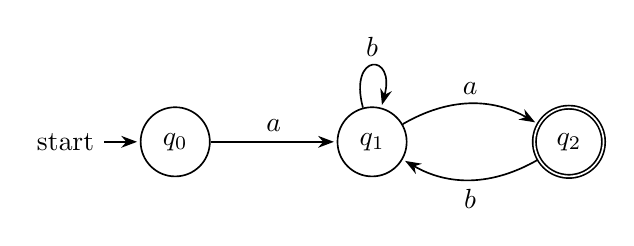
\begin{tikzpicture}[x=1cm, y=1cm]
  \begin{scope}[shift={(1.77,-1.33)}, ->, >=Stealth, shorten >=1pt, auto, node distance=2.5cm, semithick]
    \node[state, initial] (q0) at (0,0) {$q_0$};
    \node[state] (q1) at (2.5,0) {$q_1$};
    \node[state, accepting] (q2) at (5,0) {$q_2$};
    \path (q0) edge node {$a$} (q1)
          (q1) edge [loop above] node {$b$} ()
          (q1) edge [bend left] node {$a$} (q2)
          (q2) edge [bend left] node {$b$} (q1);
  \end{scope}
\end{tikzpicture}
\end{document}
